\chapter{Hydrogen}
\label{chap:h2}
    \section{Motivation}
        Hydrogen is an extremely important ingredient in many industries including fertilizers, petroleum, aerospace as rocket fuel and energy as an alternative fuel source \cite{Jacobsen2007}. Additionally, the properties of mixtures of hydrogen and other gases are also important in several other fields ranging from metrology (H$_{\rm 2}$ + H$_{\rm 2}$O) \cite{Hodges2004} to astrophysics (H$_{\rm 2}$ + He) \cite{Boothroyd2002,Boothroyd2003} to superfluidics \cite{Patkowski2008,Grebenev2000}. Therefore, computing really precise and accurate physical properties of hydrogen is vital to several industries as well as research institutions.

        Historically, hydrogen has been, and still is, one of the most studied compounds in quantum chemistry owing to its extremely simple electronic structure comprising of just one electron. Molecular hydrogen exists in two forms with significantly different physical properties \cite{Jacobsen2007}: 1) parahydrogen with anti-parallel nuclear spins and 2) orthohydrogen with parallel nuclear spins. Hydrogen also has two isotopes Deuterium (D) and Tritium (T) with 1 and 2 neutrons respectively. Several studies \cite{Goodwin1963,Kolos1986,Schwenke1988,Mielke2002,Manzhos2010,Garberoglio2010,Garberoglio2012,Sakoda2012,Garberoglio2013,Garberoglio2014} (both computational as well as experimental) of different combinations of the hydrogen molecule and its isotopes ($\allowbreak {\rm H_2, H_3, (H_2)_2, (H_2)_3, HD, HT, D_2, T_2}$ etc.) have been performed to gain further insight into the nature of interactions of these systems. However, for the purpose of evaluating fully quantum virial coefficients using \abinitio{} potentials, we restrict our attention primarily to the hydrogen dimer ${\rm (H_2)_2}$ and consider both the rigid as well as flexible monomer cases.

    \section{Recent Developments}
        In this section, we give an overview of some the \abinitio{} \PESs{} that have been developed for studying the hydrogen dimer and in the interest of brevity, we restrict our discussion to the \PESs{} that were developed on or after the year 2000.\\

        Diep and Johnson's \cite{Diep2000} pioneering work lead not only to the development of the PIMC method but also two \abinitio{} \PESs{} for the dimer with rigid monomers. One using the vibrationally-averaged bond length of the dimer and another using a slightly smaller equilibrium value, in order to study the effect of bond lengths on the \PESs{}. 37 unique angular configurations were used in the construction of these \PESs{} (and their corresponding spherical harmonics fits) and electron correlation effects were accounted at the MP2, MP3, MP4 and CCDS(T) levels of theory. They observed excellent agreement of their calculated second virial coefficient values with experiments for T = 15 to 500K. They also concluded that the differences observed in the \PESs{} based on different bond lengths were small. Boothroyd et al. \cite{Boothroyd2002} reported a rigid monomer PES (Ad) that was fit to \Sim{} 48 000 \abinitio{} energies out of which \Sim{} 42 000 were computed using the MRD-CI program of Buenker and Peyerimhoff \hl{include other papers as well} \cite{Buenker1974}. They observed significant improvement over previous \PESs{} in terms of its rms error. Robert J. Hinde \cite{Hinde2008} reported a six dimensional PES that included monomer flexibility as well and used it for studying the IR and Raman transition energies. Patkowski et al. \cite{Patkowski2008} reported a rigid monomer PES that was computed at the CCSD(T) level of theory using very large orbital basis sets. They reported second virial coefficients that were in better agreement with experiments than previous \PESs{}. It was also found that including quantum effects becomes important at \Sim{} 200K for PIMC calculations of virial coefficients. Most recently, Van and Deiters \cite{Tat2015} have reported a new \abinitio{} PES at the CCSD(T) level of theory and observed very good agreement of their calculated virial coefficients with experimental results (where available).
    \section{Computational details}
        We performed calculations for three different models of H$_2$, differing primarily in their treatment of the intramolecular bond:

        Model 1 ($s_1$): We use the rigid inter-molecular potential due to Patkowski et al.\cite{Patkowski2008} (denoted as V$_{pat}$), with the H-H bond length fixed at all temperatures to the ground state value $r_0 (= $1.448736 Bohr, same as in \cite{Patkowski2008}). Due to nonphysical energies returned by V$_{pat}$ at small inter-molecular separations, an artificial spherical hard core (with a diameter $d = 1${\AA}) is used.

        Model 2 ($s_2$): We use the flexible inter-molecular potential due to Garberoglio et al.\cite{Garberoglio2012} (denoted as V$_{hp}$), with a fixed but temperature-dependent H-H bond length, computed at each temperature to its average value $\left< r \right>_T$ (see Sec. \ref{sec:novel algorithms} for details). For V$_{hp}$, instead of an artificial spherical hard core, the potential is calculated with an inter-molecular distance $R$ which is the larger of ($R,\: 1.4${\AA}) and a bond length $b$ which is the smaller of ($b,\: 1.2${\AA}).

        Model 3 ($s_3$): We use V$_{hp}$ and allow the bond length value to vary during the calculation. The intra-molecular potential that we use is due to Mielke et al.\cite{Mielke2002} who fitted the data of Kolos et al.\cite{Kolos1986} to obtain a ground state potential.

        Mayer sampling Monte Carlo was used to sample the intermolecular distance, while the direct methods described above were used to sample path-integral image position, orientations and (where appropriate) bond lengths. It should be noted that these different MC moves were chosen with equal probability within each simulation. We ran simulations at 33 temperatures going from $T =$ 15 K $\to$ 2000 K to compare our $s_1, s_2$ and $s_3$ results against Garberoglio et al.\cite{Garberoglio2014}. We ran additional simulations at 53 temperatures going from $T =$ 16 K $\to$ 423.15 K for which experimental $B_2$ values were reported in Goodwin et al.\cite{Goodwin1963}. Although the $B_2$ values in \cite{Garberoglio2014} were calculated after choosing $P$ as a function of $T$, we ran calculations for $P = 8, 16, 32$ and $64$ for all temperatures considered because we wanted to assess the performance of the algorithms. For each value of $P$, we used a total of $10^7$ samples to evaluate the virial coefficient using the MSMC\cite{Singh2004} method. We divide the $10^7$ samples into $10^4$ blocks of $10^3$ samples each and compute block averages for the different quantities prescribed by MSMC. Using the $10^4$ block-averages, we calculate the overall averages and their standard error, and use error propagation formulas to arrive at the final uncertainties (reported here) of the virial coefficients. A reference hard sphere diameter of 3{\AA} was used for all simulations.
        Note that all simulations performed for the conditions mentioned above, were to compute the Boltzmann contribution to the virial coefficient using only Boltzmann-type configuration samples. Additionally, we also performed simulations, for each of the cases mentioned above, to compute the exchange contribution to the virial coefficient using only exchange-type configuration samples. We combine the two contributions according to their ratio as given in Fig. 2 of Garberoglio et al. \cite{Garberoglio2014} to compute the final virial coefficient values reported here. Since the ratio was zero for $T > 225$K, suggesting that exchange contributions were negligible at higher temperatures, we evaluated the exchange contributions only for temperatures $T \le 225 K$. Since the values of ratios we used were basically read off their graph and then fitted to different temperatures, there is a certain amount of random human error, for $T \le 225 K$, in the final virial coefficient results, for all Models.
    \section{Results and discussion}
        Presented below are the results of our virial coefficient calculations as a function of temperature. Since H$_2$ was considered as a test case, we tried to reproduce previous results of Garberoglio et al.\cite{Garberoglio2014} who reported second virial coefficients using VEGAS\cite{Lepage1972} algorithm for models $s_1, s_2$ and $s_3$. Hence, we just compare our values with theirs(for \emph{para}-H$_2$) as a reference for the sake of simplicity (for other literature values and/or experimental data, the interested reader may see references\cite{Goodwin1963, Patkowski2008, Leachman2009, Sakoda2012, Garberoglio2012, Garberoglio2014}). Henceforth, by ``reference values", we mean the values reported in \cite{Garberoglio2014} under similar conditions.

        We have also evaluated the performance in terms of percentage of moves accepted for both the orientation and the bond length algorithms. We have shown the same as a function of temperature for the different simulation options mentioned above.

        \subsection{Rigid-bond models: Orientation trials}
            In this section we examine the results for Models 1 and 2, which are the rigid-bond models, by which we scrutinize the validity and performance of the orientation-sampling trial, by itself. We begin by noting that the number of images used by Garberoglio for achieving converged results \cite{Patkowski2008} for Model 1 was calculated as:
            \begin{equation}
            \label{eq:s1P}
                P = 3600 K/T
            \end{equation}

            According to Eq. \eqref{eq:s1P} the temperature at which we require $P > 64$ to achieve converged results for Model 1 is 50 K. We also note that we have used a maximum of $P = 64$ images for all temperatures. Therefore we expect to see significant differences between our virial coefficient values for Model 1 and the corresponding reference values for $T \le 50 K$.

            Similarly, we have for Model 2 \cite{Garberoglio2012}:
            \begin{equation}
            \label{eq:s2P}
                P = \lceil 2500 K/T + 7 \rceil
            \end{equation}
            where $\lceil x \rceil$ denotes the smallest integer larger than $x$.

            According to Eq. \eqref{eq:s2P} the temperature at which we require $P > 64$ to achieve converged results for Model 2 is 40 K. Therefore we expect to see significant differences between our virial coefficient values for Model 2 and the corresponding reference values for $T \le 40 K$. Although for a given temperature $T$, Eqs. \eqref{eq:s1P} and \eqref{eq:s2P} provide a good estimate of $P$ required for achieving converged results, in practice, one might be able to achieve convergence with fewer $P$ as well.

            \subsubsection{Second Virial Coefficients}
                \begin{figure}[!htbp]
                    \centering
                    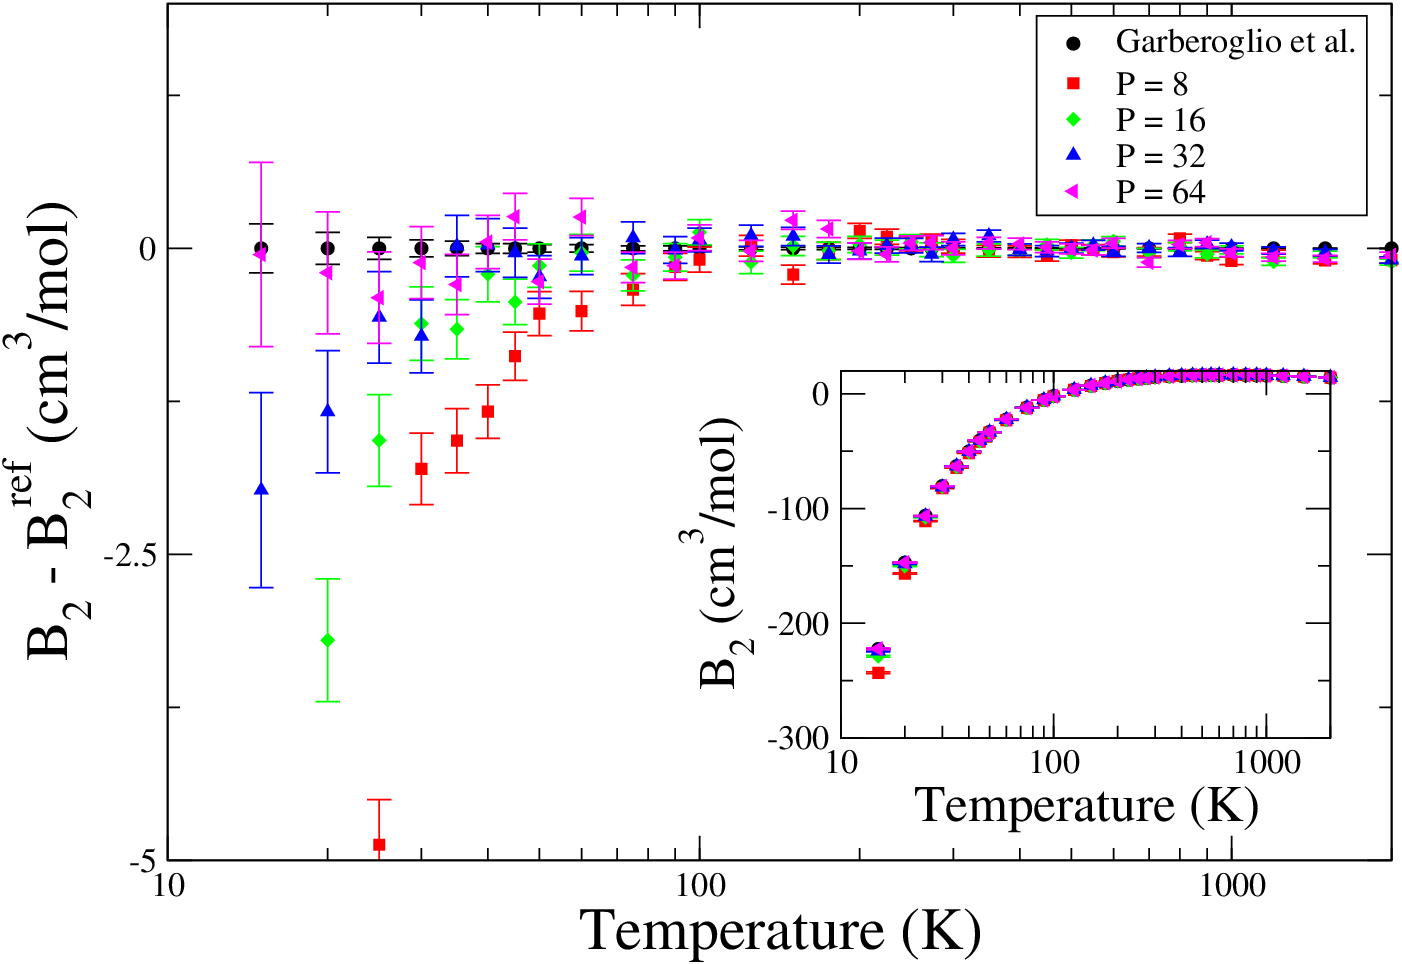
\includegraphics[width=10cm,keepaspectratio]{Chapter-4/Figures/s1GarberoglioAll.png}
                    \caption{Fully quantum second virial coefficient ($B_2$) values compared against reference values \cite{Garberoglio2014}, for Model 1. Main figure is the difference between the values computed here and the reference values, while the inset shows the coefficients before differencing. The value of the number of path-integral beads is $P$, and the results for different $P$ are as indicated in the legend. Error bars are drawn at $\mu \pm \sigma$ where $\mu$ is the mean value and $\sigma$ is the standard error. It should be noted however, that the 95\% confidence interval is given by $\mu \pm 2\sigma$.}
                    \label{fig:r0}
                \end{figure}
                In Fig. \ref{fig:r0} we show our $B_2$ values and the reference values for Model 1 as a function of temperature. It can be seen that the agreement between reference values and our results is generally good over the wide range of temperatures considered (15 K to 2000 K). The agreement is particularly good for $T > 50 K$ where our results using $P = 64$ images are sufficient enough to achieve convergence according to Eq. \eqref{eq:s1P}. For $T \le 50 K$, we observe statistically significant disagreement between our results (for all $P$ considered) and reference values and the magnitude of this deviation decreases with increasing $P$ and/or $T$ and vice-versa. As explained earlier, this behavior is expected because the number of images we use is not sufficient for convergence according to Eq. \eqref{eq:s1P}. It should be noted that in Fig. \ref{fig:r0} the range of the $y$-axis was chosen to highlight the differences over the whole range of temperatures considered and as a result we did not include some data points (whose $B_2$ value was lesser than -5 cm$^3$/mol), especially for low temperatures. However, these data points are for lower-$P$ cases where the virial coefficient values have not yet converged and so we could afford to exclude them from the graphs.

                \begin{figure}[!htbp]
                    \centering
                    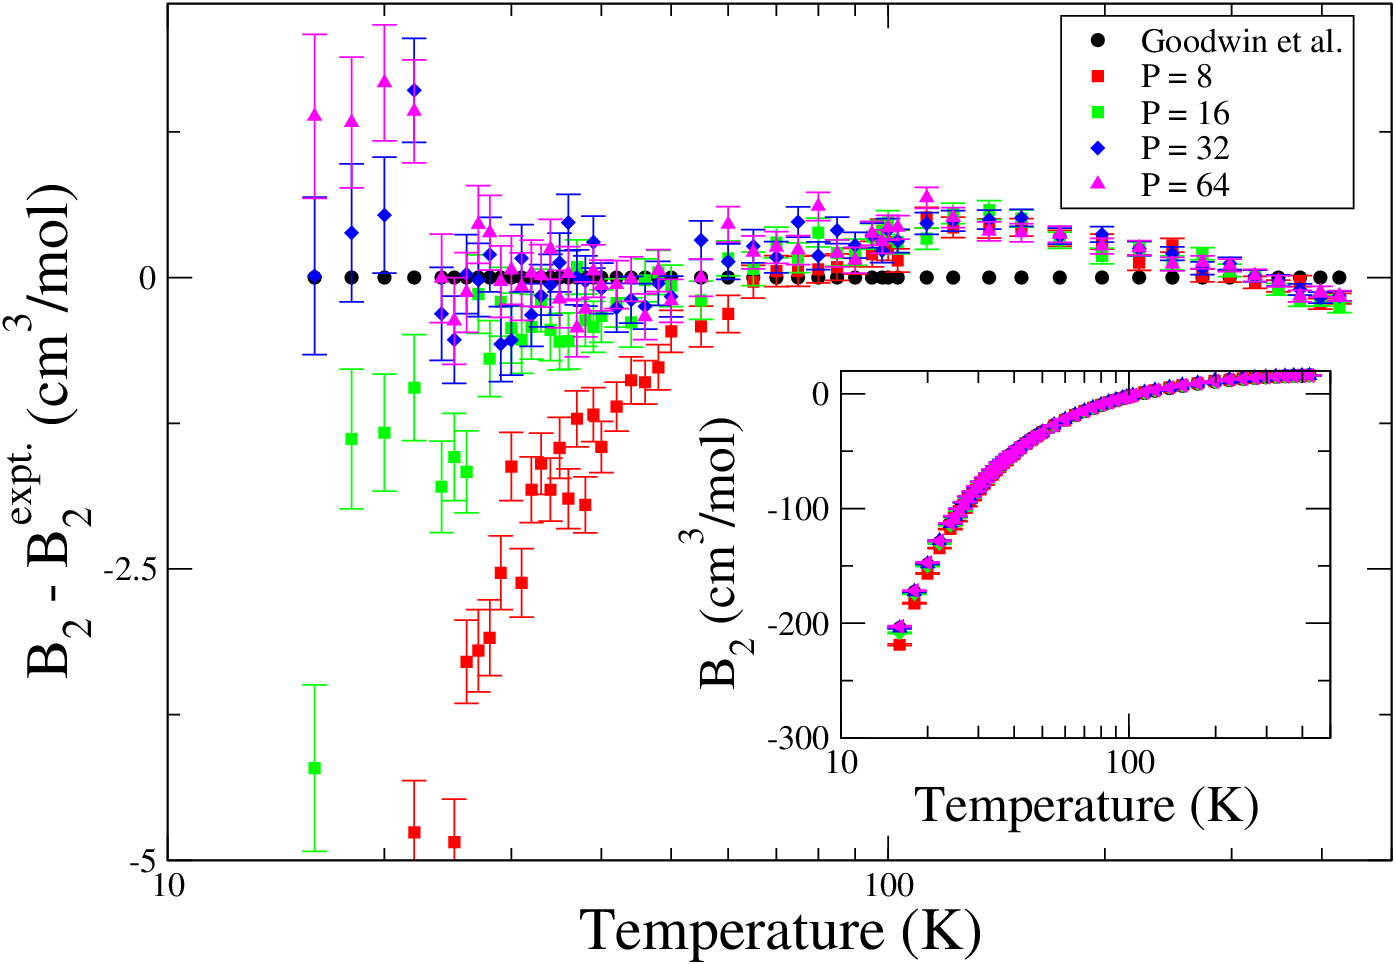
\includegraphics[scale=0.20,keepaspectratio]{Chapter-4/Figures/s1GoodwinAll.png}
                    \caption{Same as Fig. \ref{fig:r0}, but with comparison made to experimental data of Goodwin et al.\cite{Goodwin1963} rather than computed values from \cite{Garberoglio2014}.}
                    \label{fig:r0Goodwin}
                \end{figure}
                In Fig. \ref{fig:r0Goodwin} we compare our $B_2$ values for Model 1 against experimental results of Goodwin et al.\cite{Goodwin1963}. We observe particularly good agreement in two ranges of temperatures, $24 K \le T \le 50 K$ and $ 248.15 K \le T \le 423.15 K$, and significant deviations for other temperatures. Since we expect our results to have not converged for $T \le 50 K$, we consider the agreement in the range $24 K \le T \le 50 K$ to be fortuitous. At the higher temperature range where our results are converged according to Eq. \eqref{eq:s1P}, the agreement is of course expected. One possible reason for the disagreement observed at higher temperatures could be due to poor quality of the function fitted to experimental data at these temperatures. The disagreement observed at lower temperatures can be attributed to calculations involving insufficient $P$. It should be noted that in Fig. \ref{fig:r0Goodwin} the range of the $y$-axis was chosen to highlight the differences over the whole range of temperatures considered and as a result we did not include some data points (whose $B_2$ value was lesser than -5 cm$^3$/mol), especially for low temperatures. However, these data points are for lower-$P$ cases where the virial coefficient values have not yet converged and so we could afford to exclude them from the graphs.

                \begin{figure}[!htbp]
                    \centering
                    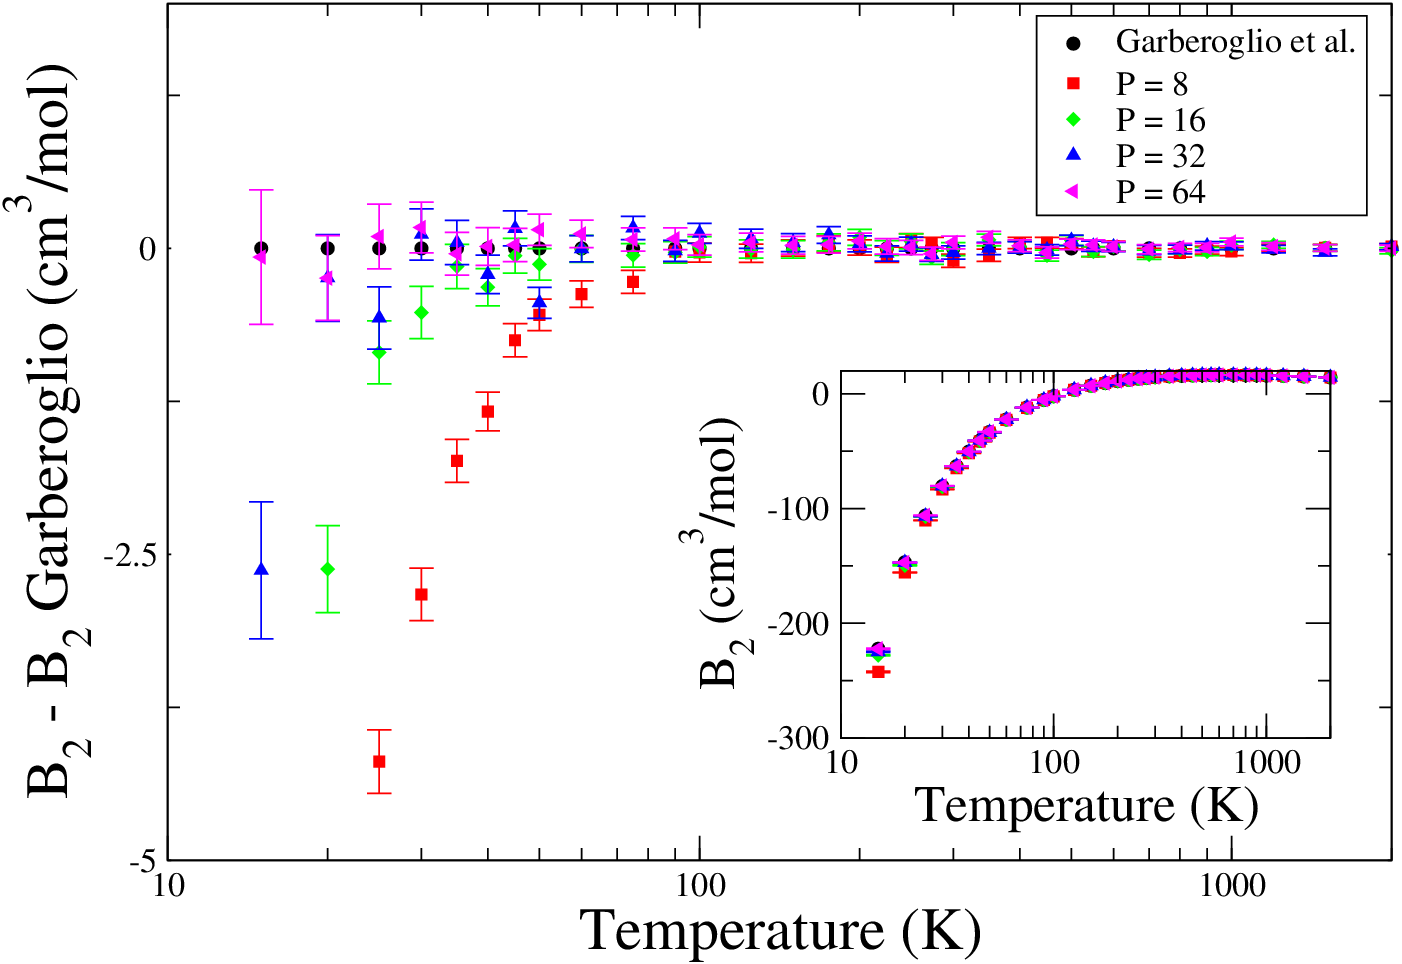
\includegraphics[scale=0.20,keepaspectratio]{Chapter-4/Figures/s2GarberoglioAll.png}
                    \caption{Same as Fig. \ref{fig:r0}, but values shown are those computed for Model 2 rather than Model 1.}
                    \label{fig:rT}
                \end{figure}
                In Fig. \ref{fig:rT} we show our $B_2$ values and the reference values for Model 2 as a function of temperature. It can be seen that the agreement between reference values and our results is particularly good for all temperatures except $T = 15 K$ and $25 K$ where our results have not converged (in accordance with Eq. \eqref{eq:s2P}). For a few temperatures below 40 K, we point out that our results have converged using fewer $P$ than that prescribed by Eq. \eqref{eq:s2P}. It should be noted that in Fig. \ref{fig:rT} the range of the $y$-axis was chosen to highlight the differences over the whole range of temperatures considered and as a result we did not include some data points (whose $B_2$ value was lesser than -5 cm$^3$/mol), especially for low temperatures. However, these data points are for lower-$P$ cases where the virial coefficient values have not yet converged and so we could afford to exclude them from the graphs.

            \subsubsection{Orientation algorithm performance}
                \label{sec:orPerformance}
                \begin{figure}[!htbp]
                    \centering
                    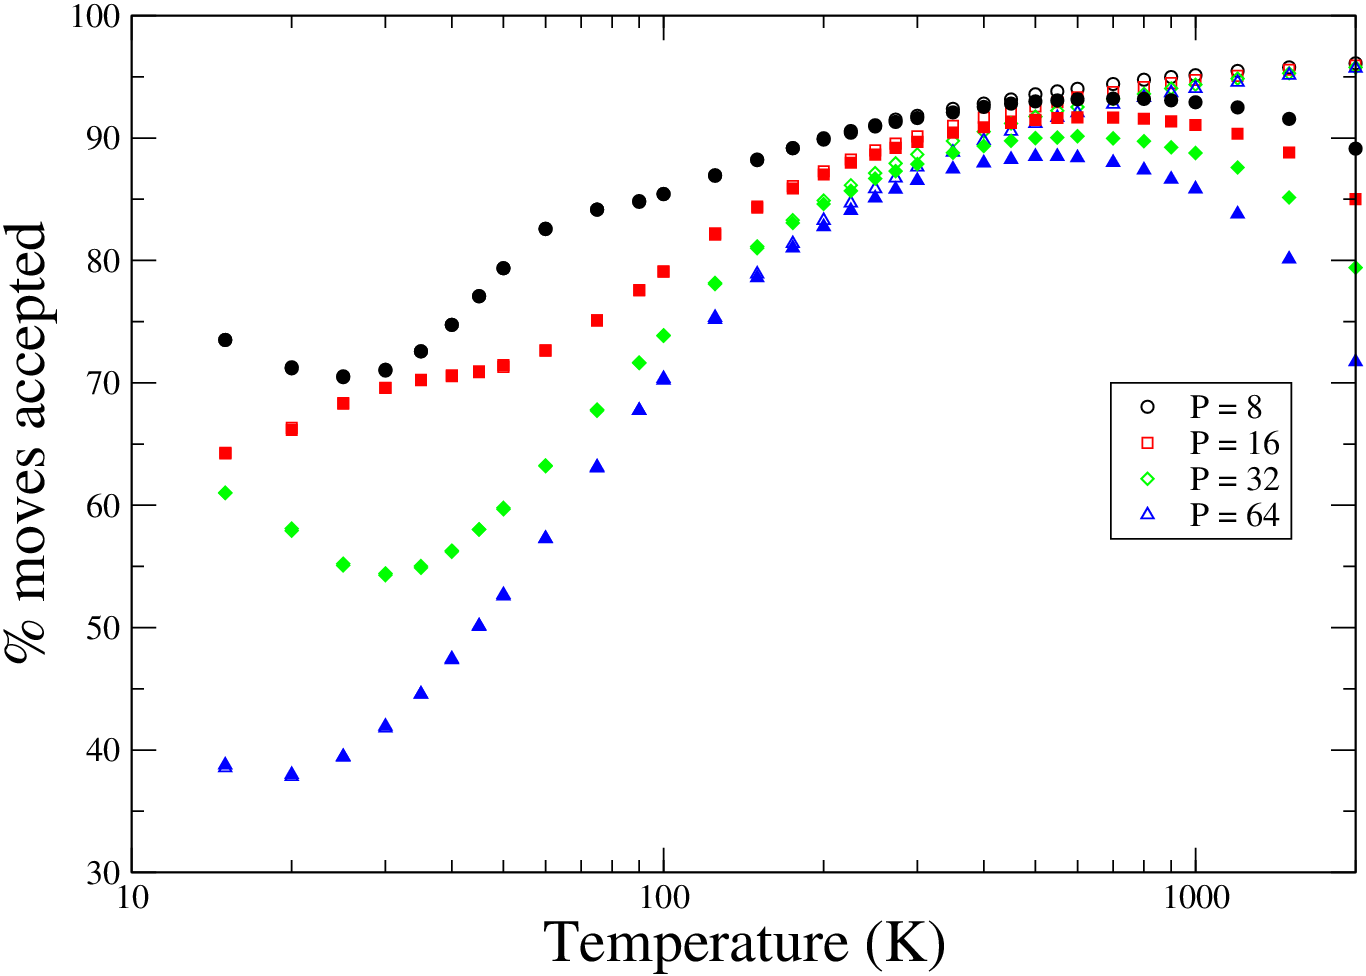
\includegraphics[scale=0.20,keepaspectratio]{Chapter-4/Figures/s12orAcc.png}
                    \caption{Performance of the orientation move for simulation options $s_1$ and $s_2$. Values for $s_1$ are represented using open symbols while that for $s_2$ are represented using filled symbols with the same shape.}
                    \label{fig:r0Acc}
                \end{figure}

                In fig. \ref{fig:r0Acc} we show the percentage of orientation moves that were accepted as a function of temperature for simulation options $s_1$ and $s_2$. Although we require more $P$ to accurately capture the nuclear quantum effects at low temperature, the efficiency of the algorithm decreases with increasing $P$ as is evident in the figure. As explained earlier, this is because we achieve exact sampling of the angle $\alpha$ only for the $P/2$ images that are placed in the last step of the orientation algorithm. For the other $P/2$ images, the sampling is approximate and not exact. Still, the acceptance rate at all conditions is quite good, and in the worst case hovers around 40\%, which means that roughly two attempts at generating a configuration are required to produce one that is acceptable. Given that the new configuration is completely uncorrelated from the one preceding it, this represents a significant improvement in the efficiency of sampling of the path-integral conformations.

                It is worth noting that in fig. \ref{fig:r0Acc}, there is a significant change in the behavior of the curves for $s_1$ and $s_2$, only for temperatures $\ge$ 700 K, where the performance for the $s_1$ case is increasing while that of $s_2$ is decreasing. To explain this phenomena and gain further insight into the nature of the difference between the actual distribution $\pi({\mathbf b})$ (Eq. \eqref{eq:piTotal}) and the approximate distribution $\tilde\pi({\mathbf b})$ (Eq. \eqref{eq:piTilde}), we ran simulations for a few hypothetical conditions and collected histograms of the angle between image 0 and image $P'$. We generated configurations by setting $P' = $ 2 and $k_h = $ 0.5 \AA$^{-2}$, and adjusting the simulation temperature accordingly (to hypothetical values). After choosing uniformly random orientations for all images as part of a MC trial, we accept or reject the trail based on $\pi ({\mathbf b})$ (Eq. \eqref{eq:piTotal}). We noted in Sec. \ref{subsec:orMove} that the ratio of the actual and approximate distribution for any image $j$ would be farthest from 1 for the first step of the algorithm. Therefore the histogram farthest away from $\pi ({\mathbf b})$, for the angle between the same set of images can be evaluated analytically using the approximate distribution function and assuming image $P'$ was placed in the first step (i.e., using Eq. \eqref{eq:piTildebj} with $j = P'$ and $\psi = 0$). By comparing these two histograms, we were able to visualize the nature of difference between the two distributions qualitatively. We repeated the above exercise for $P' =$ 4, 8 and $k_h =$ 5 \AA$^{-2}$, 50 \AA$^{-2}$ and their different permutations as well. It should be noted that all histograms were collected using 100 bins and 10$^8$ samples each.

                \begin{figure}[!htbp]
                    \centering
                    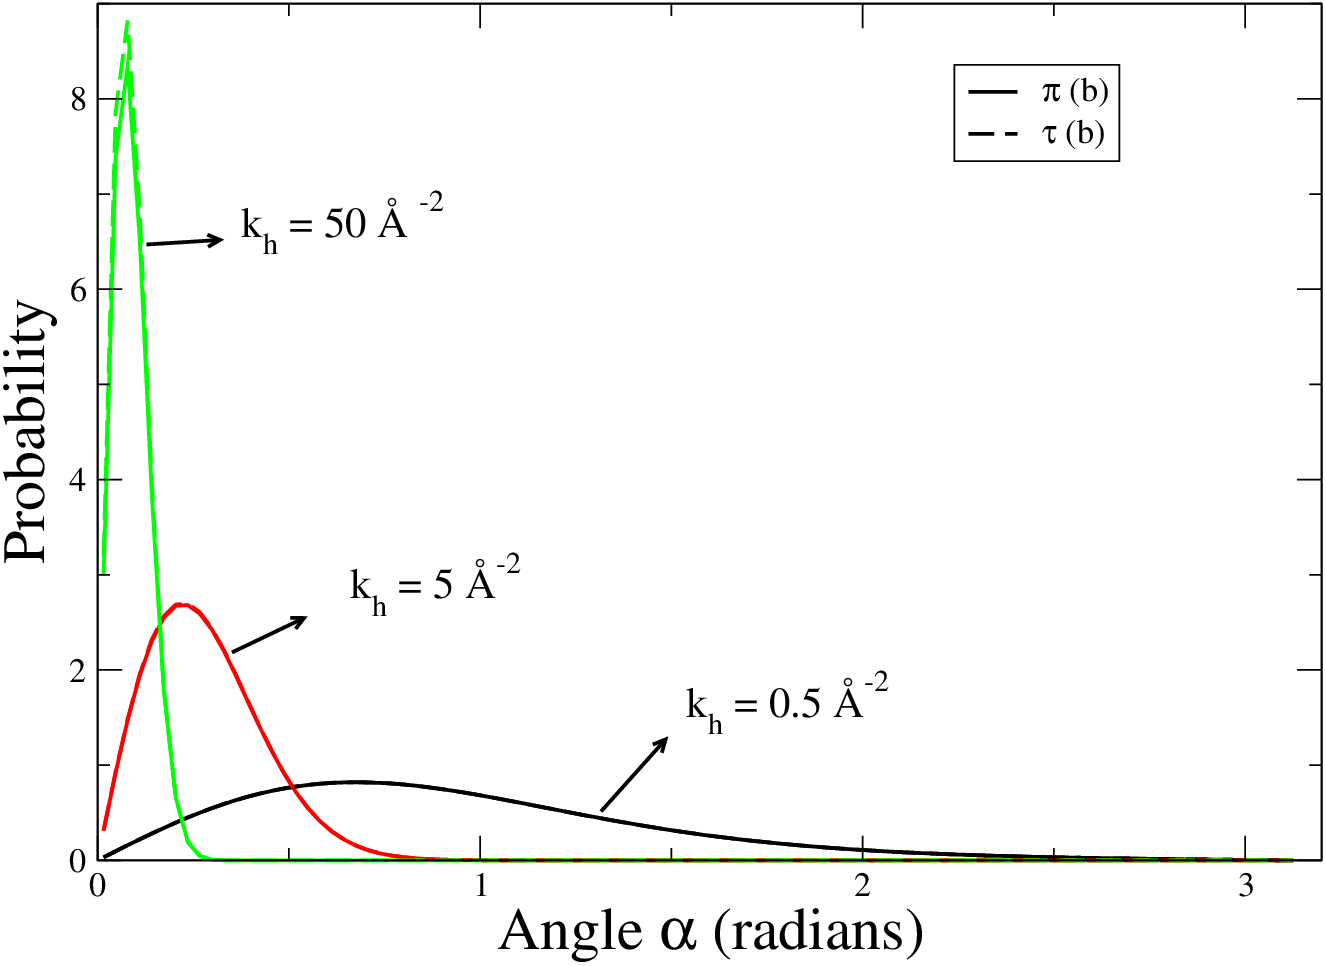
\includegraphics[scale=0.20,keepaspectratio]{Chapter-4/Figures/phi2B.png}
                    \caption{Approximate and actual probability distributions for $P' =$ 2.}
                    \label{fig:phi2B}
                \end{figure}

                \begin{figure}[!htbp]
                    \centering
                    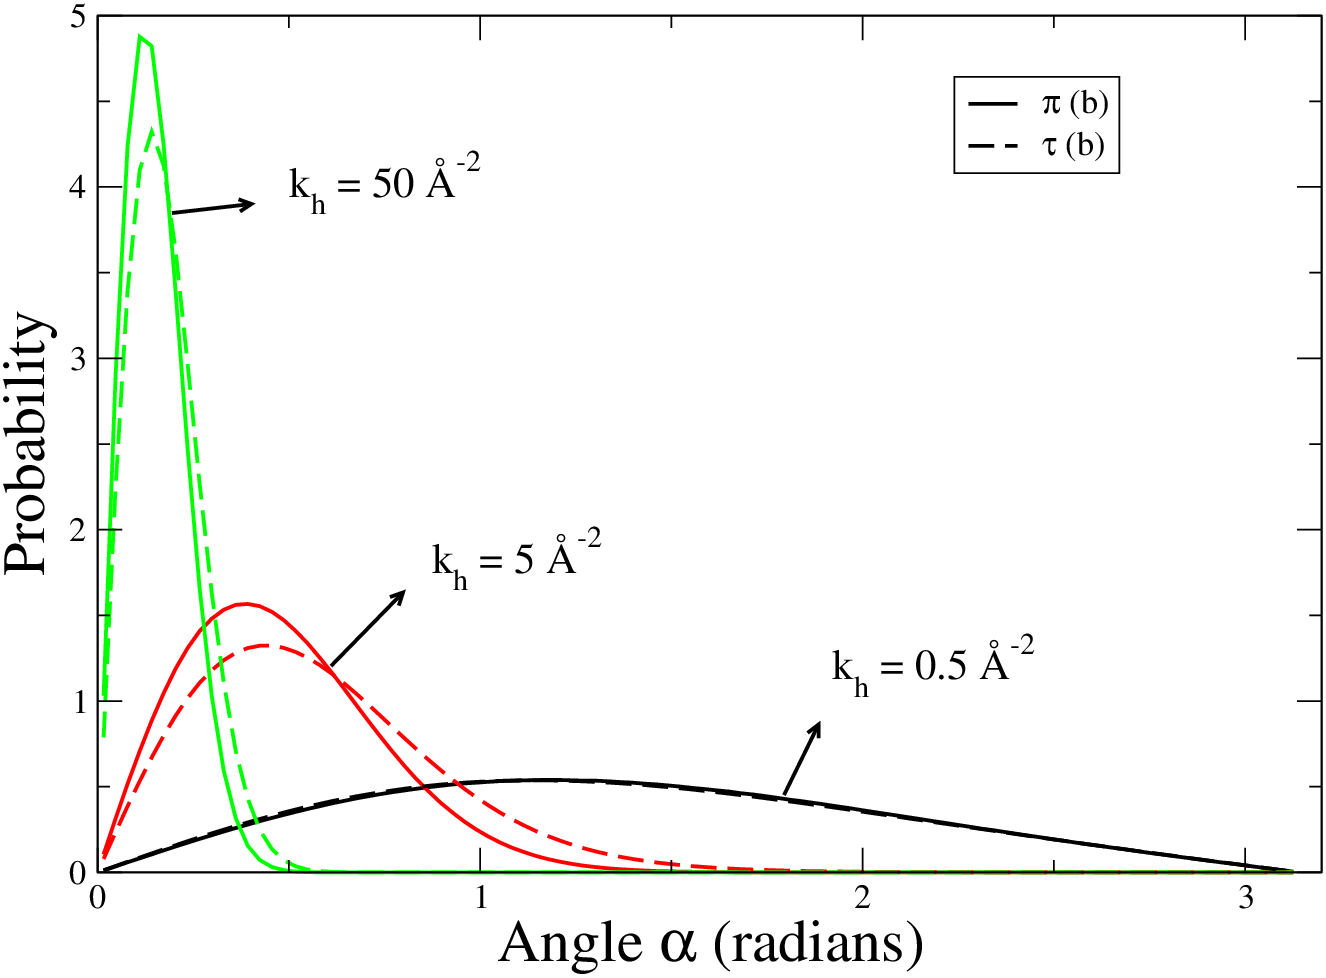
\includegraphics[scale=0.20,keepaspectratio]{Chapter-4/Figures/phi4B.png}
                    \caption{Approximate and actual probability distributions for $P' =$ 4.}
                    \label{fig:phi4B}
                \end{figure}

                \begin{figure}[!htbp]
                    \centering
                    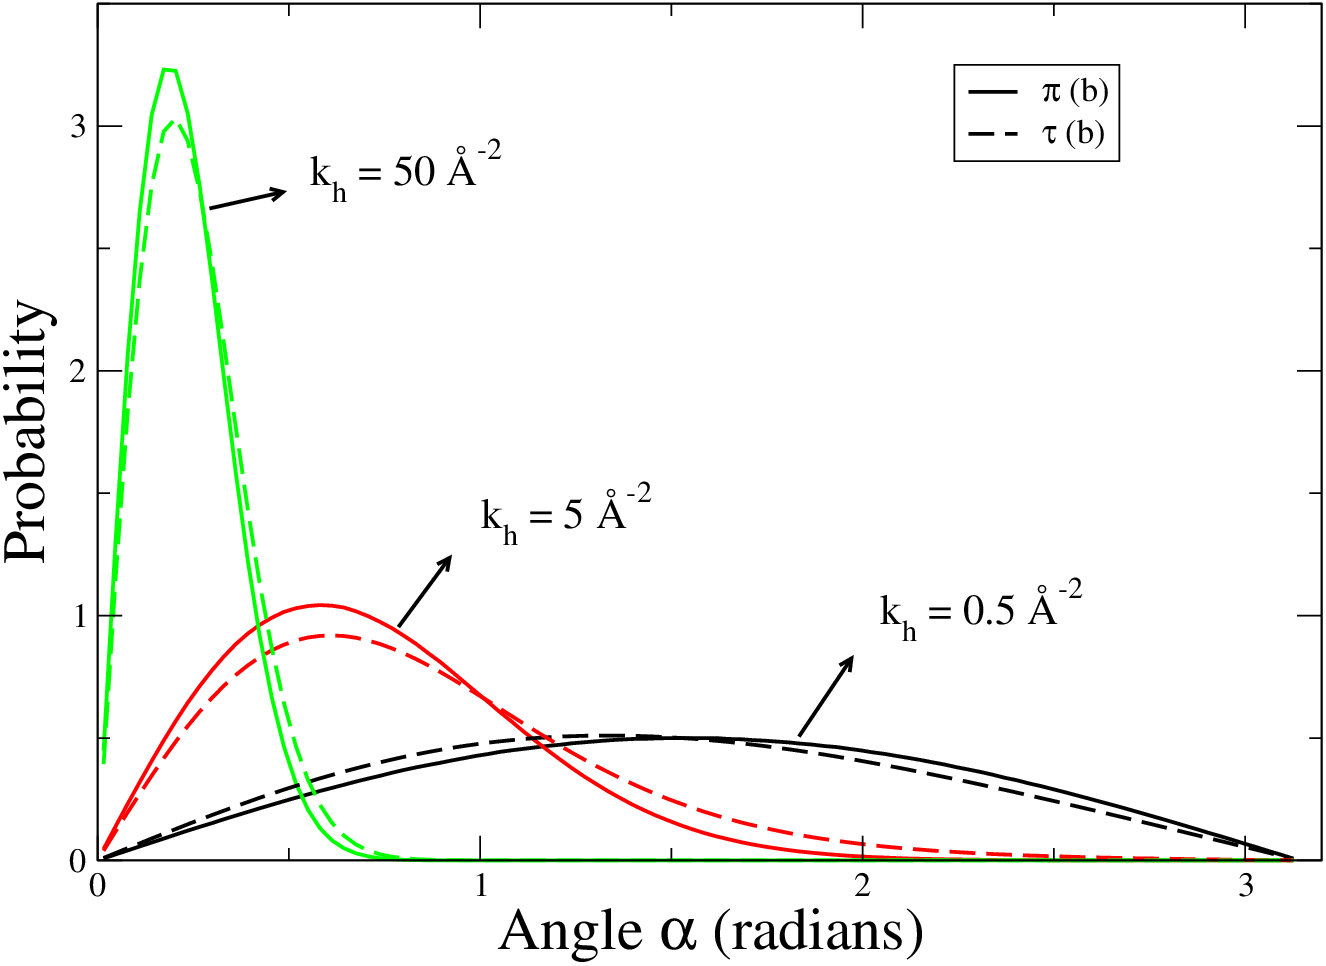
\includegraphics[scale=0.20,keepaspectratio]{Chapter-4/Figures/phi8B.png}
                    \caption{Approximate and actual probability distributions for $P' =$ 8.}
                    \label{fig:phi8B}
                \end{figure}

                From figs. \ref{fig:phi2B}, \ref{fig:phi4B} and \ref{fig:phi8B}, we can infer the following:
                \begin{itemize}
                    \item For a given $P$, we observe that the approximate distribution seems to be under-predicting for some range of angles and over-predicting for other ranges, as it must for both distributions to be normalized.
                    \item For a given $P$, the actual distribution gets narrower and taller as we increase $k_h$. This is to be expected because springs with high $k_h$ values tend to prefer smaller angles $\alpha$ as they are harmonically more favorable. The generally increasing trend in the percentage moves accepted as a function of temperature (as seen in fig. \ref{fig:r0Acc}) can be explained due to this phenomenon.
                \end{itemize}

                To further elucidate the difference between the approximate and actual distributions, we plot the ratio of the actual and the approximate distributions on the $y$-axis and the approximate distribution on the $x$-axis for the different hypothetical conditions mentioned above. For ease of explanation, we define ``closeness" between the two distributions as the deviation of $y$-coordinate from the $y =$ 1-line in figs. \ref{fig:ratio2B}, \ref{fig:ratio4B} and \ref{fig:ratio8B}.

                \begin{figure}[!htbp]
                    \centering
                    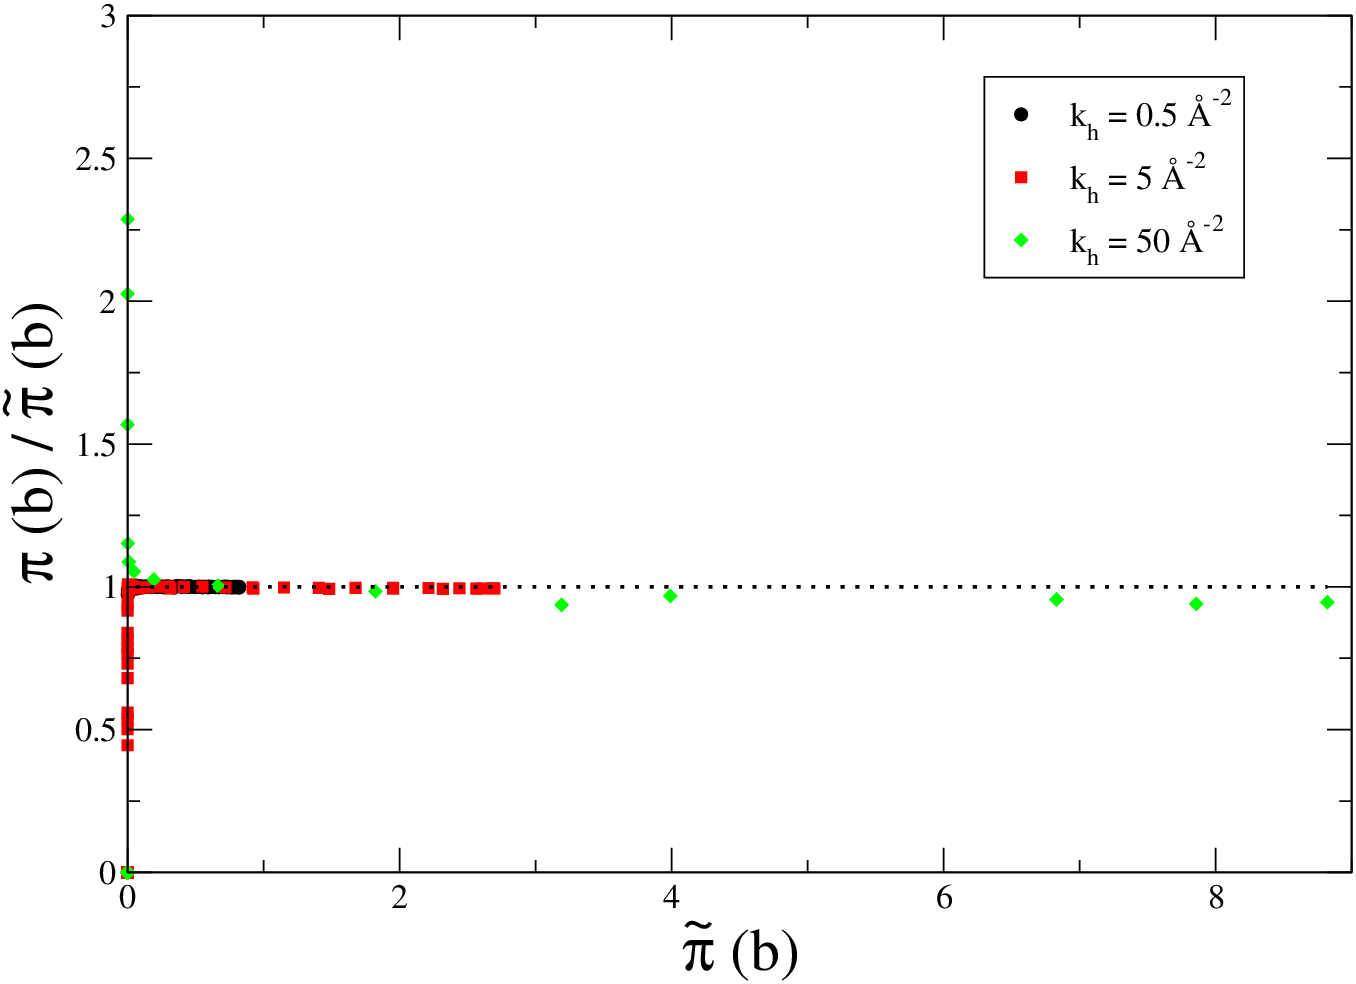
\includegraphics[scale=0.20,keepaspectratio]{Chapter-4/Figures/ratio2B.png}
                    \caption{Ratio of the approximate and actual probability distributions for $P' =$ 2.}
                    \label{fig:ratio2B}
                \end{figure}

                \begin{figure}[!htbp]
                    \centering
                    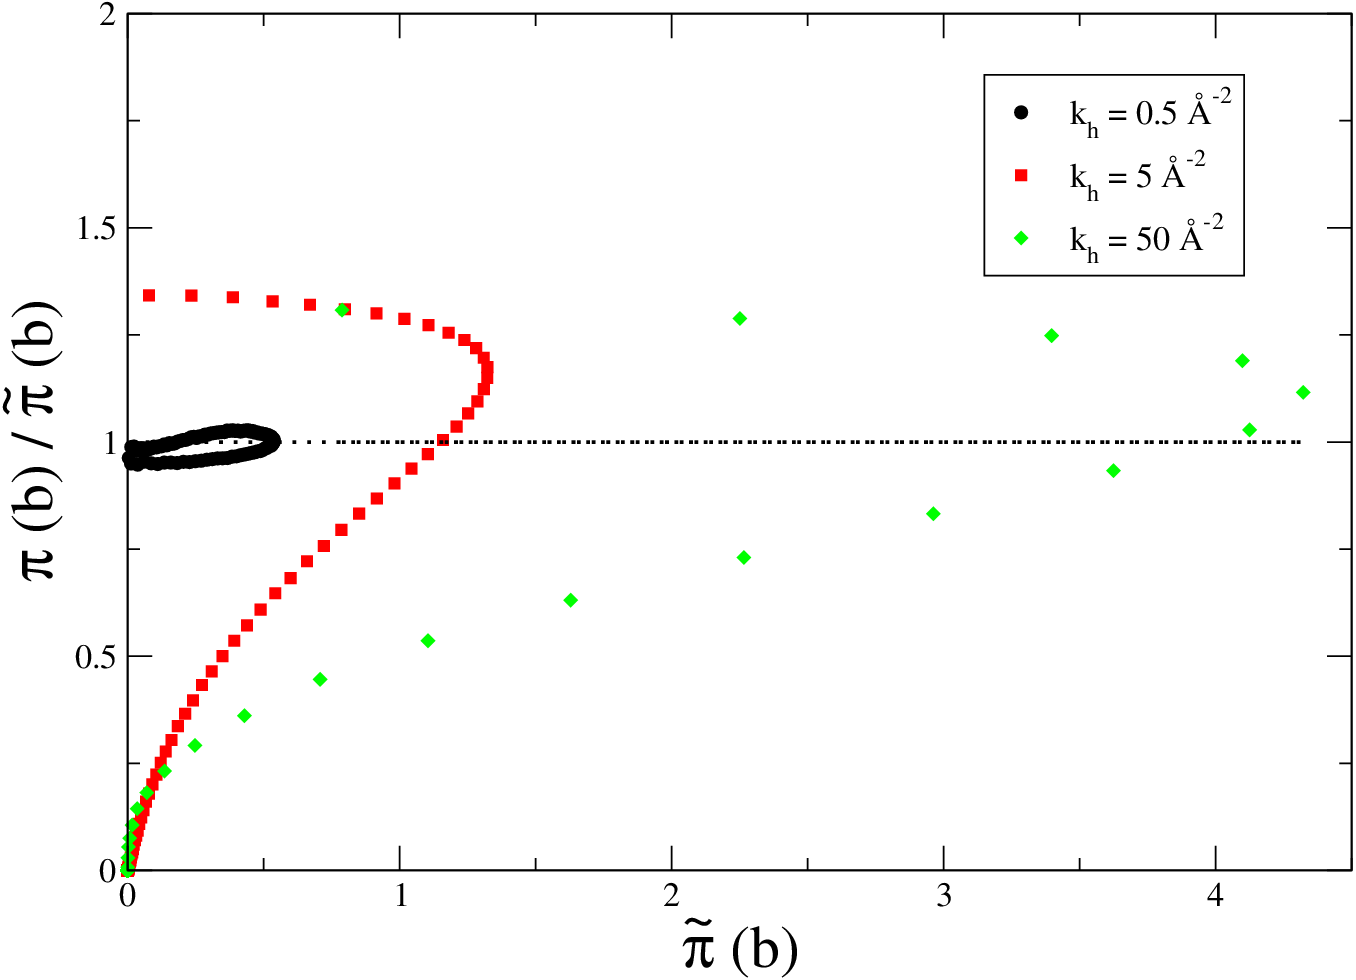
\includegraphics[scale=0.20,keepaspectratio]{Chapter-4/Figures/ratio4B.png}
                    \caption{Ratio of the approximate and actual probability distributions for $P' =$ 4.}
                    \label{fig:ratio4B}
                \end{figure}

                \begin{figure}[!htbp]
                    \centering
                    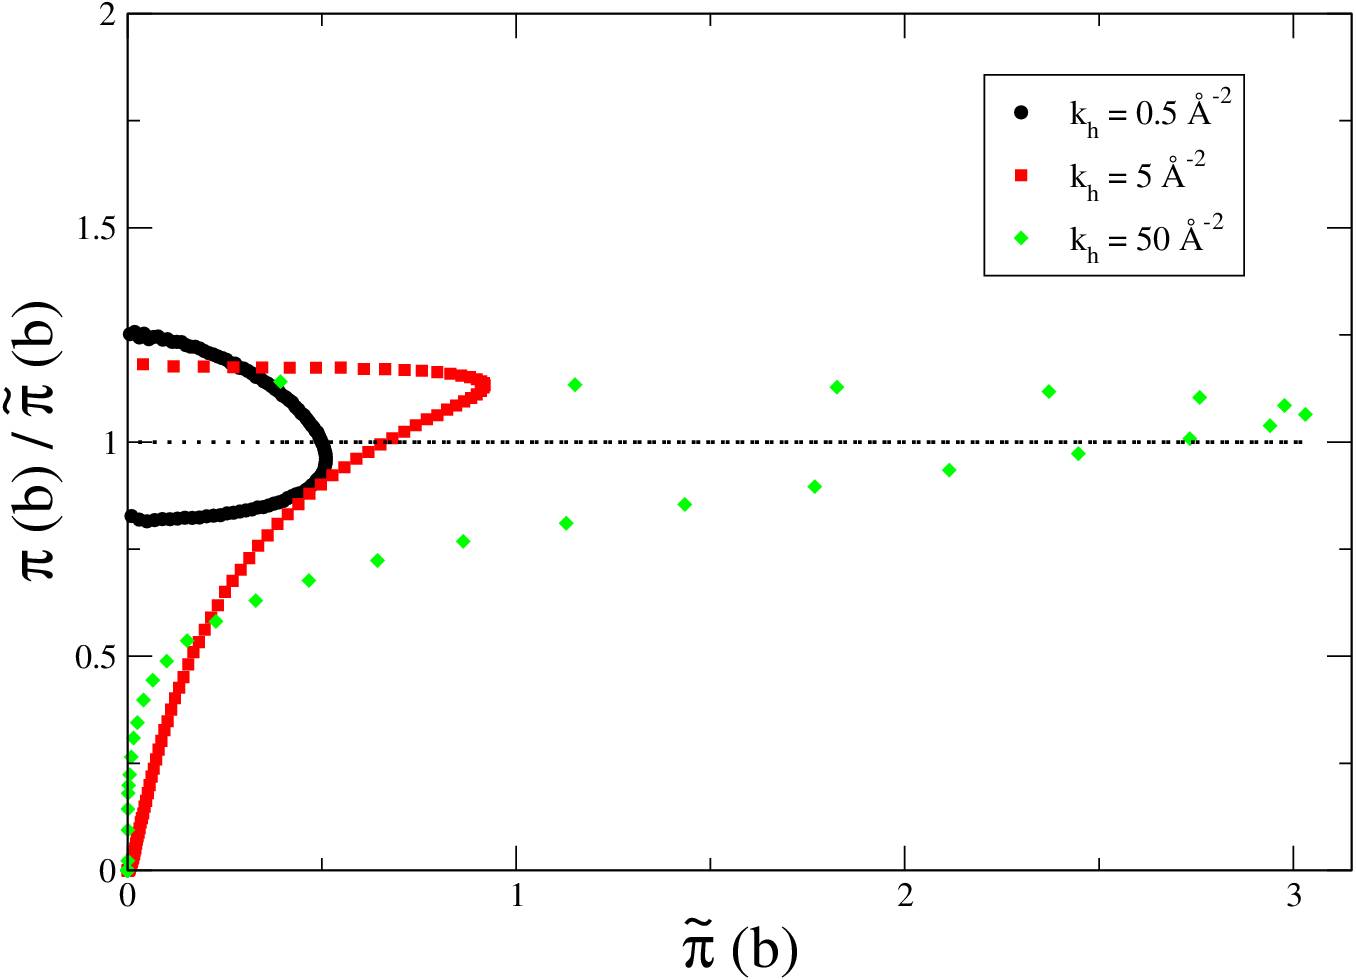
\includegraphics[scale=0.20,keepaspectratio]{Chapter-4/Figures/ratio8B.png}
                    \caption{Ratio of the approximate and actual probability distributions for $P' =$ 8.}
                    \label{fig:ratio8B}
                \end{figure}

                From figs. \ref{fig:ratio2B}, \ref{fig:ratio4B} and \ref{fig:ratio8B}, we can infer the following:
                \begin{itemize}
                    \item In some cases, ``closeness" (as defined above) of the intermediate $k_h$ (= 5 \AA$^{-2}$) is worse than the other two cases. This could lead to the minimum in fig. \ref{fig:r0Acc} because $k_h$ is directly proportional to temperature. It is worth noting that although for one particular image the approximate distribution could be very ``close" to the actual distribution, as we take the product of many such approximate distribution functions the resulting probability distribution function is worse than each individual approximate.
                    \item The points above the $y =$ 1-line indicate  that the actual distribution has been under-predicted by the approximate distribution and these points could potentially lead to configurations where the molecule is `stuck'. In other words, the probability of going from one of these points to a point on the $y =$ 1-line (favored) is very poor. However, this would happen only for $y \gg 1$, which is not observed in any of the hypothetical cases.
                \end{itemize}

        \subsection{Flexible-bond models: Orientation and bond length trials}
            In this section we present and analyze the results for Model 3 (flexible-bond model) including the performance of the orientation-sampling trial and the bond length sampling trial when present simultaneously in a simulation. We begin by noting that the number of images used by Garberoglio for achieving converged results \cite{Garberoglio2014} for Model 3 was calculated as:
            \begin{equation}
            \label{eq:s3P}
                P = \lceil 7000 K/T + 8 \rceil
            \end{equation}
            where $\lceil x \rceil$ denotes the smallest integer larger than $x$.

            According to Eq. \eqref{eq:s3P} the temperature at which we require $P > 64$ to achieve converged results for Model 3 is 100 K. Therefore we expect to see significant differences between our virial coefficient values for Model 3 and the corresponding reference values for $T \le 100 K$. Although for a given temperature $T$, Eq. \eqref{eq:s3P} provides a good estimate of $P$ required for achieving converged results, in practice, one might be able to achieve convergence with fewer $P$ as well.

            \subsubsection{Second Virial Coefficients}
                \begin{figure}[!htbp]
                    \centering
                    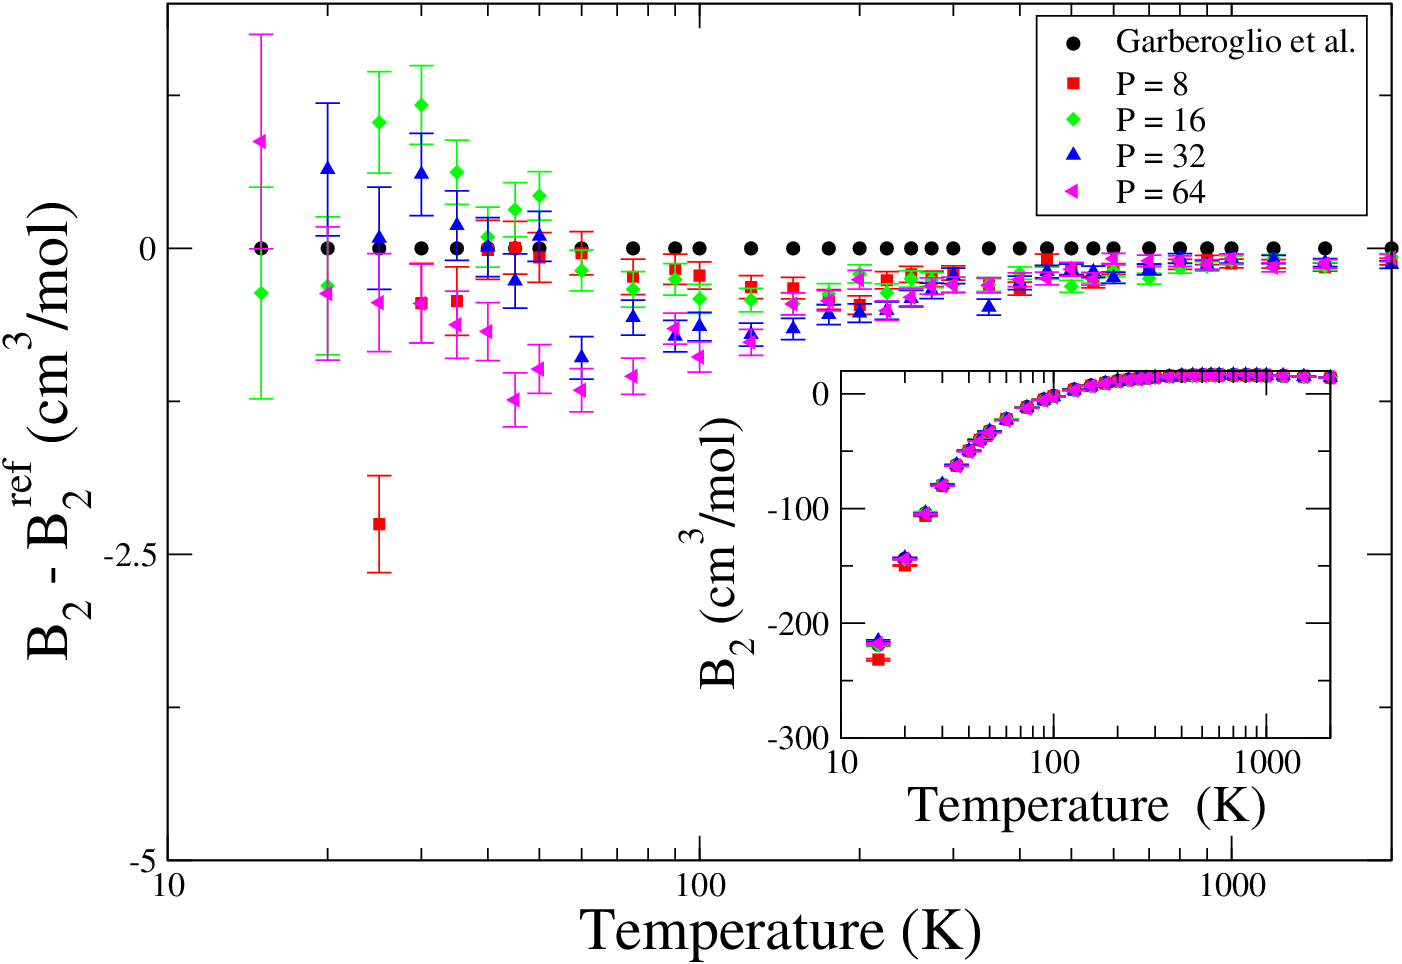
\includegraphics[scale=0.20,keepaspectratio]{Chapter-4/Figures/s3GarberoglioAll.png}
                    \caption{Fully quantum second virial coefficient ($B_2$) values compared against reference values \cite{Garberoglio2014}, for Model 3. Main figure is the difference between the values computed here and the reference values, while the inset shows the coefficients before differencing. The value of the number of path-integral beads is $P$, and the results for different $P$ are as indicated in the legend. Error bars are drawn at $\mu \pm \sigma$ where $\mu$ is the mean value and $\sigma$ is the standard error. It should be noted however, that the 95\% confidence interval is given by $\mu \pm 2\sigma$.}
                    \label{fig:variable}
                \end{figure}

                In Fig. \ref{fig:variable} we show our $B_2$ values and the reference values for Model 3 as a function of temperature. It can be seen that the agreement between reference values and our results is generally good over the wide range of temperatures considered (15 K to 2000 K). The agreement is particularly good for $T > 100 K$ where our results using $P = 64$ images are sufficient enough to achieve convergence according to Eq. \eqref{eq:s3P}. For $T \le 100 K$, we observe statistically significant disagreement between our results (for all $P$ considered) and reference values and the magnitude of this deviation decreases with increasing $P$ and/or $T$ and vice-versa. As explained earlier, this behavior is expected because the number of images we use is not sufficient for convergence according to Eq. \eqref{eq:s3P}. It should be noted that in Fig. \ref{fig:r0} the range of the $y$-axis was chosen to highlight the differences over the whole range of temperatures considered and as a result we did not include some data points (whose $B_2$ value was lesser than -5 cm$^3$/mol), especially for low temperatures. However, these data points are for lower-$P$ cases where the virial coefficient values have not yet converged and so we could afford to exclude them from the graphs.

            \subsubsection{Orientation algorithm performance}
                \begin{figure}[!htbp]
                    \centering
                    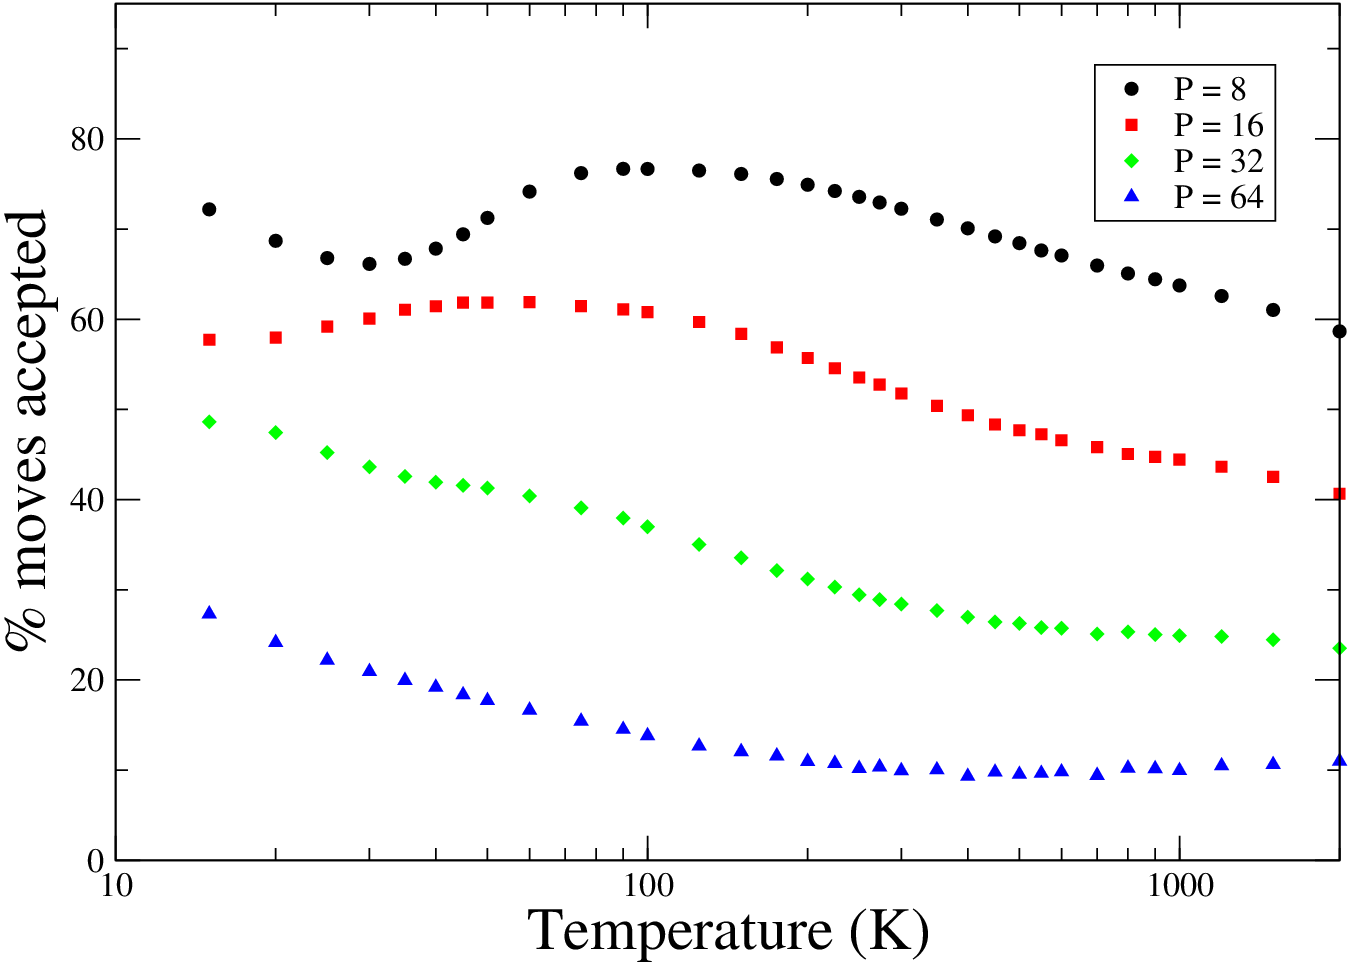
\includegraphics[scale=0.20,keepaspectratio]{Chapter-4/Figures/s3OrAcc.png}
                    \caption{Performance of the orientation move for simulation option $s_3$}
                    \label{fig:variableOrAcc}
                \end{figure}

                In fig. \ref{fig:variableOrAcc} we have shown the percentage of orientation moves that were accepted as a function of temperature for simulation option $s_3$. We notice once again that the algorithm performance decreases with increasing $P$ which is to be expected because of the non-exact nature of the description of the $\alpha$ for $P/2$ images. In addition, we also observe that the performance of the orientation move is almost always worse in the presence of the bond length change move as can be seen in figs. \ref{fig:r0Acc} and \ref{fig:variableOrAcc}. This can be attributed to the way we handle the bond lengths of different images being different within the orientation move. In its current implementation, we average the bond lengths of images $i$ through $k$ and use this value to place image $j$. However, this leads to using the incorrect value of the spring constant when computing the approximate distribution function, which in turn could lead to poor percentage acceptance of the move.

            \subsubsection{Bond length algorithm performance}
                \label{sec:blPerformance}
                Before looking at the performance of the bond length algorithm, we present the following as evidence to support our use of the expression $b_i^{2/P}$ in place of $b_i^2$ in eq. \eqref{eq:ytilde}. We collected histograms of the average adjacent angle $\theta_{ij}$ during the course of $s_1$ simulations for $T = 15, 50, 100, 250$~and $500$ K and for $P = 8, 16, 32$~and $64$.
                \begin{figure}[!htbp]
                    \centering
                    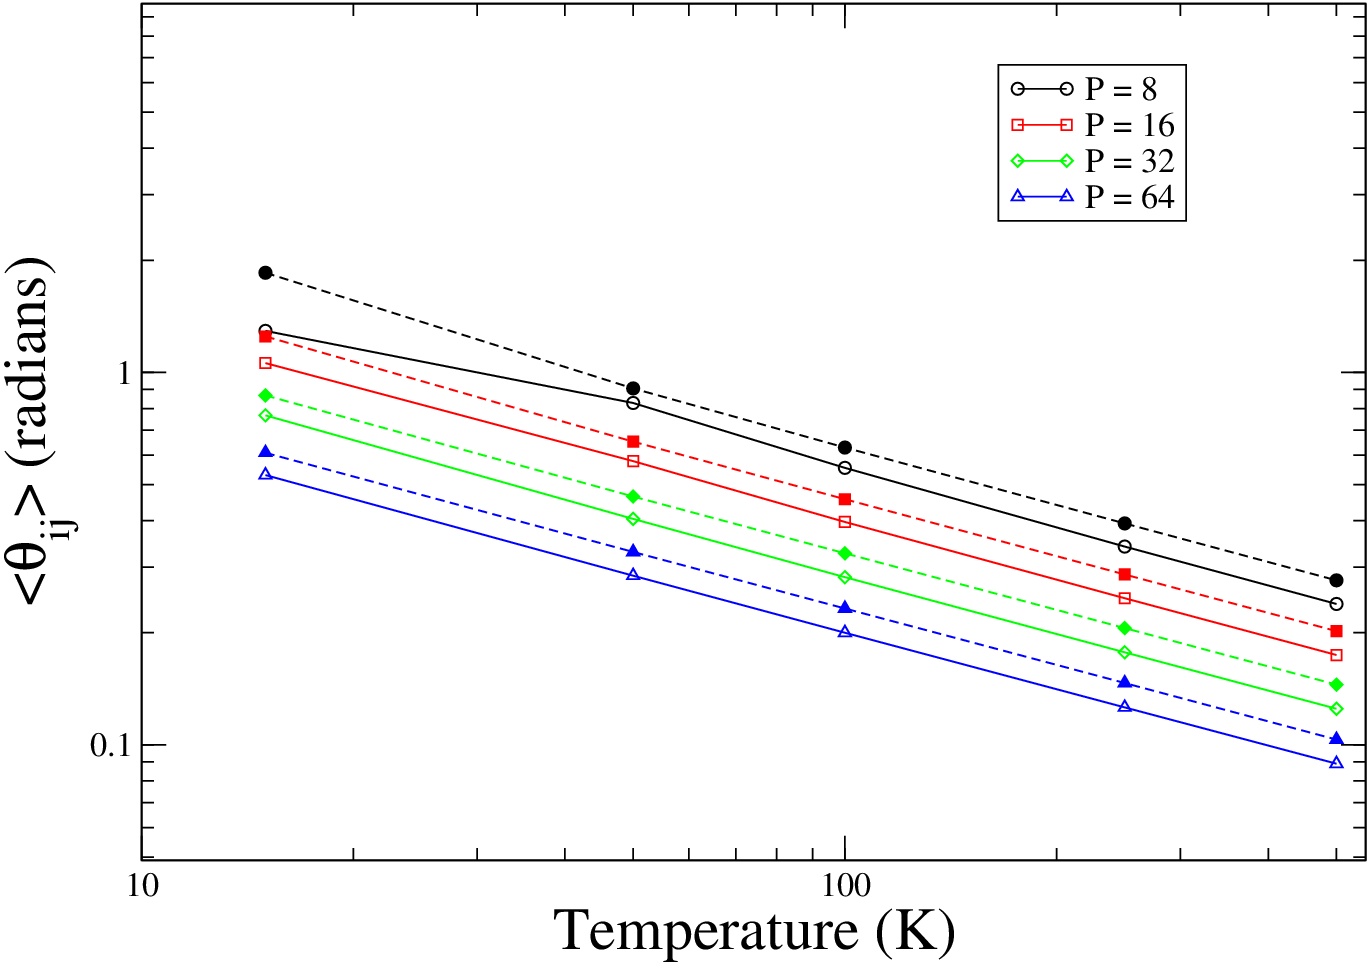
\includegraphics[scale=0.20,keepaspectratio]{Chapter-4/Figures/nominalAnglelogXlogY.png}
                    \caption{Nominal angle computed using eq. \eqref{eq:thetaHat} compared against average $\theta_{ij}$ observed in simulation (Note: both axes are shown in log scale). Open symbols connected by solid lines represent the $<\theta_{ij}>$ observed in simulation and filled symbols with the same shape connected by dashed lines represent the $\hat \theta$ computed using the formula given in eq. \eqref{eq:thetaHat}}
                    \label{fig:nominal_angle}
                \end{figure}

                From fig. \ref{fig:nominal_angle} we can clearly see that although eq. \eqref{eq:thetaHat} over-predicts $<\theta_{ij}>$ slightly for all cases, this would result only in a marginal decrease in the efficiency of the sampling algorithm. Therefore, we assumed it would be a small price to pay when compared to the amount of computational effort saved by not performing the normal mode analysis before each bond length trial.

                \begin{figure}[!htbp]
                    \centering
                    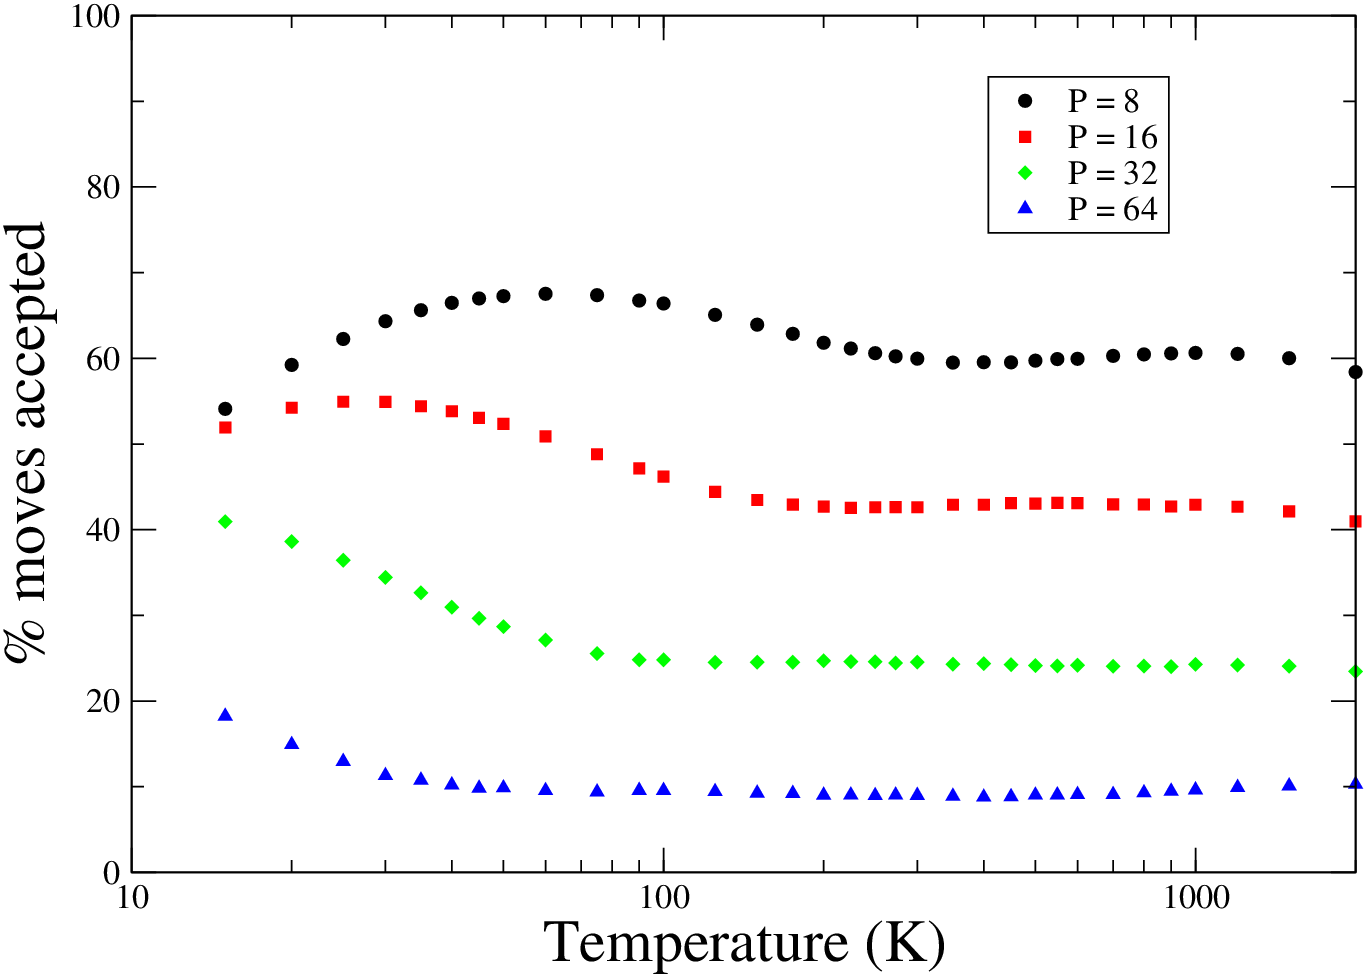
\includegraphics[scale=0.20,keepaspectratio]{Chapter-4/Figures/s3BlAcc.png}
                    \caption{Performance of the bond length move for simulation option $s_3$}
                    \label{fig:variableBlAcc}
                \end{figure}

                In fig. \ref{fig:variableBlAcc} we have shown the percentage of bond length moves that were accepted as a function of temperature for simulation option $s_3$. For a fixed $T$, the percentage acceptance decreases with increasing $P$. Although the approximation of the behavior of the bond lengths to be of Gaussian nature using the normal mode analysis affects the performance of the bond length algorithm, we did not attempt to investigate this further. Neither did we probe alternative approaches to compute the nominal angle $\hat \theta$. For our current purposes, we found the performance of the bond length sampling algorithm to be satisfactory.

                The algorithms developed in Sections \ref{subsec:orMove} and \ref{subsec:blMove} do not involve the use of quantum chemistry calculations and hence allow for considerable efficiency improvements. The mass of the atom that forms the diatomic molecule is used as input to each of the algorithms. Although this allows us to differentiate between different isotopes of the same atom, the algorithms cannot differentiate between the different quantum mechanical spins(i.e., \emph{para}- and \emph{ortho}-H$_2$) of the molecule. Garberoglio et al. \cite{Garberoglio2014} use different number of images $P$, as a means to accomplishing this difference within the PIMC calculation. We have not used the same $P$ as theirs, in order to gauge the performance of our algorithms for different conditions as mentioned above. Therefore, in some cases, we observe large deviations from reference values where the use of larger $P$ is necessary.
